\documentclass[compress]{beamer}

\mode<presentation>
{
  %\usetheme{Warsaw}
  %\usecolortheme{spruce}
  % or ...
	%\useoutertheme{infolines}
  %\setbeamercovered{transparent}
  
  \usetheme{CambridgeUS}
    \setbeamercolor{item projected}{bg=darkred}
    \setbeamertemplate{enumerate items}[default]
    \setbeamertemplate{navigation symbols}{}
    \setbeamercovered{transparent}
    \setbeamercolor{block title}{fg=darkred}
    \setbeamercolor{local structure}{fg=darkred}
  
  % or whatever (possibly just delete it)
}

\usepackage{verbatim} 
\usepackage{listings}
\usepackage{tikz}
\usetikzlibrary{arrows}
\usetikzlibrary{shapes}
\tikzstyle{block}=[draw opacity=0.7,line width=1.4cm]

\newcommand{\bigpause}{\bigskip \pause}

\lstloadlanguages{C++}
\lstnewenvironment{code}
	{%\lstset{	numbers=none, frame=lines, basicstyle=\small\ttfamily, }%
	 \csname lst@SetFirstLabel\endcsname}
	{\csname lst@SaveFirstLabel\endcsname}
\lstset{% general command to set parameter(s)
	language=C++, basicstyle=\footnotesize\sffamily, keywordstyle=\slshape,
	emph=[1]{tipo,usa}, emphstyle={[1]\sffamily\bfseries},
	basewidth={0.47em,0.40em},
	columns=fixed, fontadjust, resetmargins, xrightmargin=5pt, xleftmargin=15pt,
	flexiblecolumns=false, tabsize=2, breaklines,	breakatwhitespace=false, extendedchars=true,
	numbers=left, numberstyle=\tiny, stepnumber=1, numbersep=9pt,
	frame=l, framesep=3pt,
}

\usepackage[spanish]{babel}
% or whatever

\usepackage[utf8]{inputenc}
% or whatever

\usepackage{times}
\usepackage[T1]{fontenc}
% Or whatever. Note that the encoding and the font should match. If T1
% does not look nice, try deleting the line with the fontenc.


\title[Geometr\'ia Computacional] % (optional, use only with long paper titles)
{Geometr\'ia Computacional}

\author[Melanie Sclar] % (optional, use only with lots of authors)
{~Melanie Sclar}
% - Give the names in the same order as the appear in the paper.
% - Use the \inst{?} command only if the authors have different
%   affiliation.
\institute[UBA] % (optional, but mostly needed)
{
  %\inst{1}%
  Facultad de Ciencias Exactas y Naturales\\
  Universidad de Buenos Aires
}
\date[PAP] % (optional, should be abbreviation of conference name)
{Problemas, Algoritmos y Programación}

% Ac¿ se puede insertar el logo de la UBA
% \pgfdeclareimage[height=0.5cm]{university-logo}{university-logo-filename}
% \logo{\pgfuseimage{university-logo}}



% Delete this, if you do not want the table of contents to pop up at
% the beginning of each subsection:
\AtBeginSubsection[]
{
  \begin{frame}<beamer>{Contenidos}
    \tableofcontents[currentsection,currentsubsection]
  \end{frame}
}

\newcommand{\be}{\begin{equation*}}
\newcommand{\ee}{\end{equation*}}
\newcommand{\state}[1]{\left|\,#1\,\right\rangle}
\newcommand{\costate}[1]{\left\langle\,#1\,\right|}
\newcommand{\trace}{\text{Tr}}
\newcommand{\su}{\uparrow}
\newcommand{\sd}{\downarrow}
\newcommand{\im}{\text{Im}}
\newcommand{\re}{\text{Re}}

\newcommand{\tabu}{\hspace*{0.7cm}}
\newcommand{\ctabu}{\hspace*{0.8cm}}
\newcommand{\htabu}{\hspace*{0.25cm}}

% If you wish to uncover everything in a step-wise fashion, uncomment
% the following command:

%\beamerdefaultoverlayspecification{<+->}


\begin{document}
\pgfdeclarelayer{background}
\pgfsetlayers{background,main}
\begin{frame}
  \titlepage
\end{frame}

\begin{frame}{Contenidos}
  \tableofcontents
  % You might wish to add the option [pausesections]
\end{frame}

\section{Técnicas de barrido}

\subsection{Sweep ray}
\begin{frame}
La clase pasada vimos el algoritmo de Graham Scan para obtener la convex hull
de un conjunto de puntos. \\

\bigskip
Usaremos el mismo algoritmo para resolver algunos otros problemas.
\end{frame}

\begin{frame}

\begin{block}{Problema}
Dados $n$ puntos $p_1, \ldots p_n \in \mathbb{R}^2$, hallar la 
cantidad de triángulos obtusángulos que se pueden formar.
\end{block}

\end{frame}

\begin{frame}{Solución}
\begin{itemize}
\item Haremos un sweep ray, pero su implementación deberá ser más cuidadosa
pues debo girar $2\pi$ radianes.

\item Fijo el nodo que será el vértice correspondiente al ángulo obtuso. Ahora sólo
debo encontrar los otros dos.

\item Tengo un rayo que decide quién será el primer vértice a analizar. Luego, habrá
un intervalo de amplitud de ángulo, donde todos los nodos contenidos en 
ese intervalo son posibles terceros vértices. Cuento cuántos son en cada
instante.

\item Puedo mantener el conjunto de vértices candidatos en un $set$, y como
podemos observar un nodo será insertado y removido exactamente una vez.
\end{itemize}
\end{frame}

\begin{frame}

\begin{block}{Problema}
Dados $n$ puntos en la grilla ($p_1, \ldots p_n \in \mathbb{Z}^2$), 
hallar la cantidad de triángulos isósceles que se pueden formar.
\end{block}

\end{frame}

\begin{frame}

\begin{itemize}
\item Primero fijo un punto que será el vértice opuesto al lado diferente.
\item Ahora debo contar la cantidad de puntos a igual distancia, pues
todos ellos son posibles otros vértices del triángulo isósceles.
\item Para ello, ordeno los puntos según su distancia al centro.
\item Luego falta restar los triángulos equiláteros, que contamos varias
veces. Reflexionemos un momento acá, ¿hace falta esto?
\end{itemize}
\end{frame}

\subsection{Sweep circle}

\begin{frame}{¿Qu\'e es sweep circle?}
\begin{itemize}
\item La idea de sweep circle es exactamente la misma que la ya mencionada sweep line, pero en lugar de mover una recta imaginaria, movemos una circunferencia.

\item La circunferencia puede moverse en linea recta (traslación) o alrededor de un centro fijo (rotación).

\item Como un círculo es una figura acotada, el choque de la circunferencia con los puntos interesantes produce eventos de \textit{entrada} y de \textit{salida} en el círculo.
\end{itemize}
\end{frame}

\begin{frame}{Ejemplo: Ubicación ideal de un círculo en el eje Y}

\begin{block}{Problema}
    Dado un radio $R > 0$ entero, se debe indicar cuál es la máxima cantidad de puntos de la grilla de coordenadas enteras que es posible encerrar con un círculo de radio $R$, cuyo centro se encuentre posicionado sobre la recta $x=0$ (el eje $y$).
\end{block}

\pause
\invisible<1-1>
{
    Observación: Alcanza con considerar las posiciones $0 \leq y \leq 1$
}

\end{frame}

\begin{frame}{Planteo con sweep circle}

\begin{itemize}
    \item Comenzamos con el círculo ubicado en $(0,0)$, y todos los correspondientes puntos de la grilla adentro.
    \item ``Movemos'' el círculo en vertical, hasta llegar a $(0,1)$, procesando los eventos de entrada y salida de puntos.
    \item La máxima cantidad de puntos que tengamos dentro del círculo en cualquier momento, es el resultado.
\end{itemize}

\pause

\invisible<1-1>{
    \begin{itemize}
       \item Notar que hay solamente $O(R)$ eventos de entrada / salida, y además la cantidad de puntos totales dentro del círculo inicial puede computarse en $O(R)$.
       \item Con todo esto y la técnica de barrido, el problema se resuelve en $O(R \lg R)$
    \end{itemize}
}

\end{frame}

\begin{frame}{Problemas para pensar}

\begin{itemize}
\item goo.gl/rT7Ji
\item goo.gl/llEHC
\end{itemize}

\end{frame}

\subsection{Sweep line - problemas más complejos}
\begin{frame}{Área de unión de rectángulos}

\begin{block}{Problema}
Dados $n$ rectángulos alineados con respecto a los ejes del plano, 
¿cuál es el área de la unión de todos ellos?
\end{block}

%%%%%%%%%%% TODO %%%%%%%%%%%%%

\end{frame}

\begin{frame}

\begin{center}
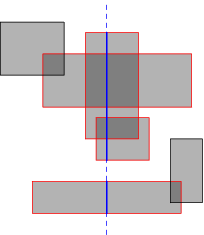
\includegraphics[scale=0.7]{images/rectangle_union.png}
\end{center}

\end{frame}

\begin{frame}

\begin{itemize}
\item Haremos un sweep line con una recta vertical, comprimiendo las coordenadas
(es decir, no reviso todos los valores de $x$ sino solo los interesantes:
los eventos). ¿Cuáles serán los eventos?
\pause
\item Los eventos serán la apertura y clausura de los rectángulos (o sea,
el borde izquierdo y derecho).
\item Va a haber un conjunto de rectángulos $vivos$, es decir, los que
se encuentran activos en el momento analizado. ¿Cuál es el área entre
el punto $i$ del sweep line y el $i+1$?
\pause
\item Como entre dos puntos consecutivos no puede haber dejado de existir
un rectángulo, el área entre esos dos cortes verticales
es $(p_{i+1} - p_i) \cdot alturas$ siendo $alturas$ la longitud
de la totalidad de los rangos (notar que si se superponen, los contamos una
sola vez).
\end{itemize}

\end{frame}

\begin{frame}{Ejemplo visual - área de unión de rectángulos}
\begin{center}
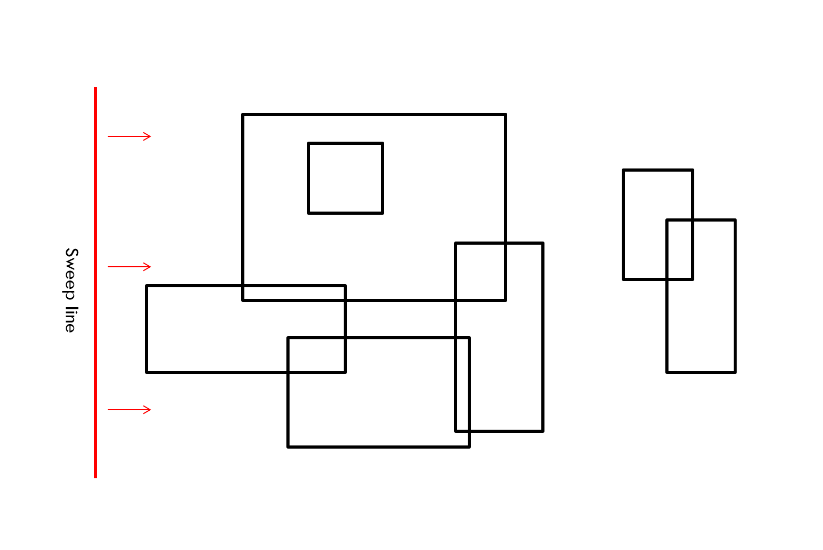
\includegraphics[scale=0.4]{images/sweep_line_1.png}
\end{center}
\end{frame}

\begin{frame}{Ejemplo visual - área de unión de rectángulos}
\begin{center}
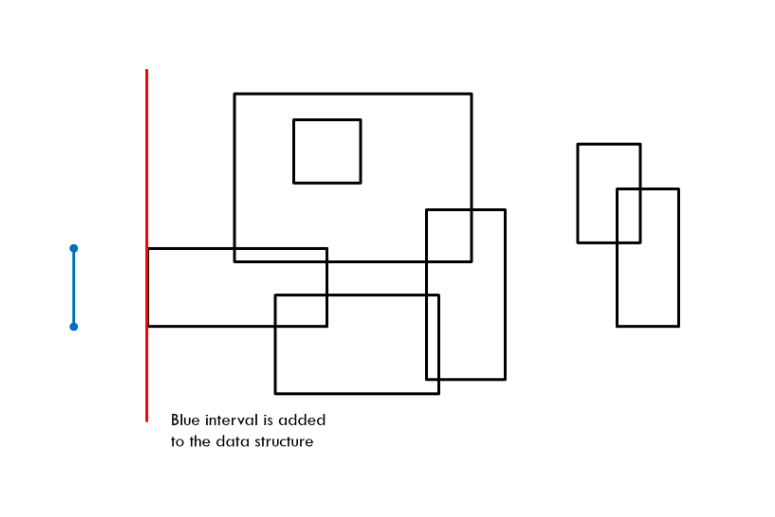
\includegraphics[scale=0.4]{images/sweep_line_2.png}
\end{center}
\end{frame}

\begin{frame}{Ejemplo visual - área de unión de rectángulos}
\begin{center}
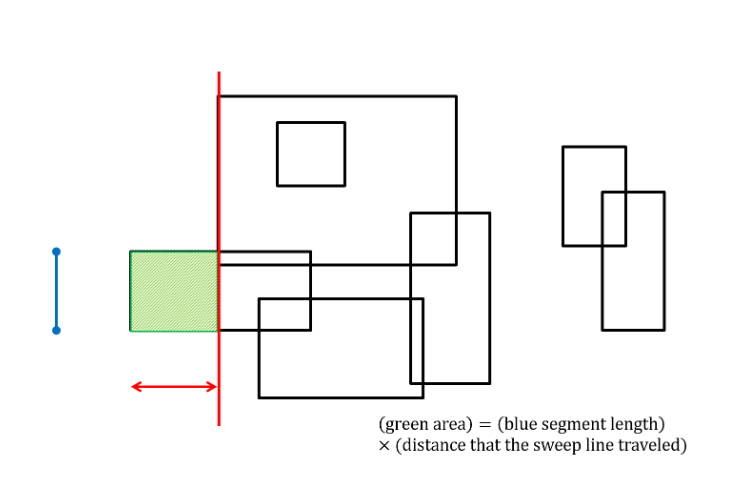
\includegraphics[scale=0.4]{images/sweep_line_3.png}
\end{center}
\end{frame}

\begin{frame}{Ejemplo visual - área de unión de rectángulos}
\begin{center}
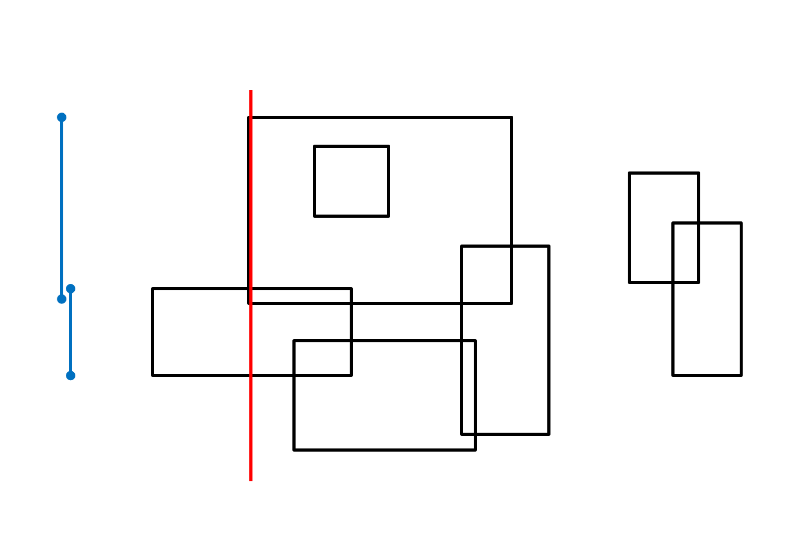
\includegraphics[scale=0.4]{images/sweep_line_4.png}
\end{center}
\end{frame}

\begin{frame}{Ejemplo visual - área de unión de rectángulos}
\begin{center}
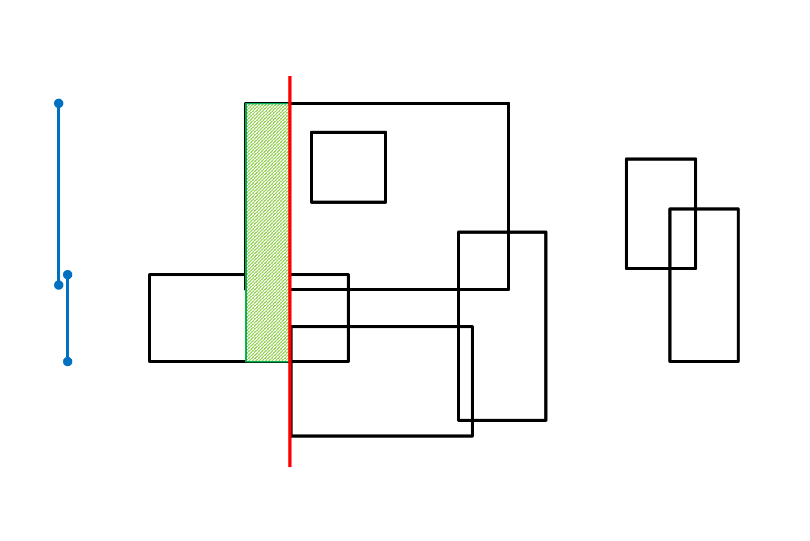
\includegraphics[scale=0.4]{images/sweep_line_5.png}
\end{center}
\end{frame}

\begin{frame}{Ejemplo visual - área de unión de rectángulos}
\begin{center}
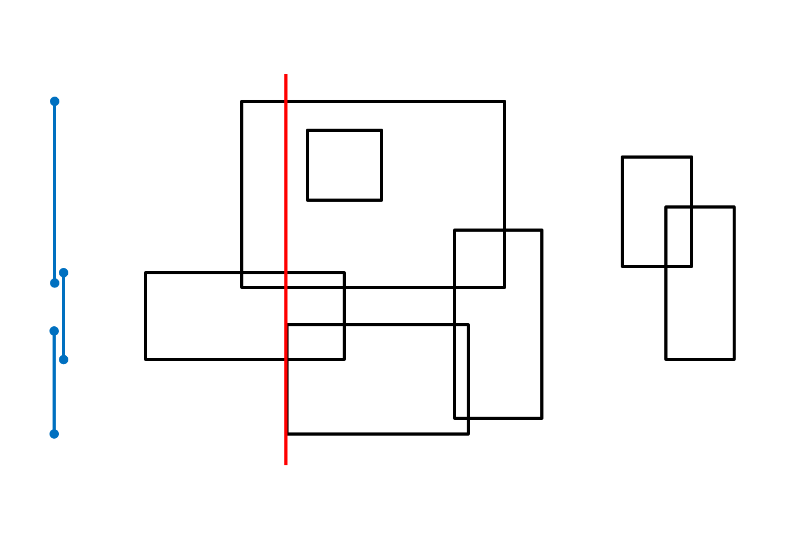
\includegraphics[scale=0.4]{images/sweep_line_6.png}
\end{center}
\end{frame}

\begin{frame}{Ejemplo visual - área de unión de rectángulos}
\begin{center}
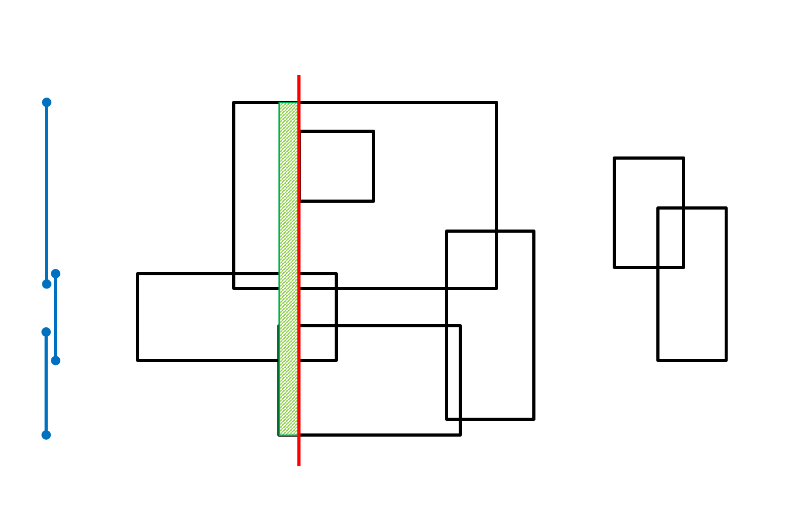
\includegraphics[scale=0.4]{images/sweep_line_7.png}
\end{center}
\end{frame}

\begin{frame}{Ejemplo visual - área de unión de rectángulos}
\begin{center}
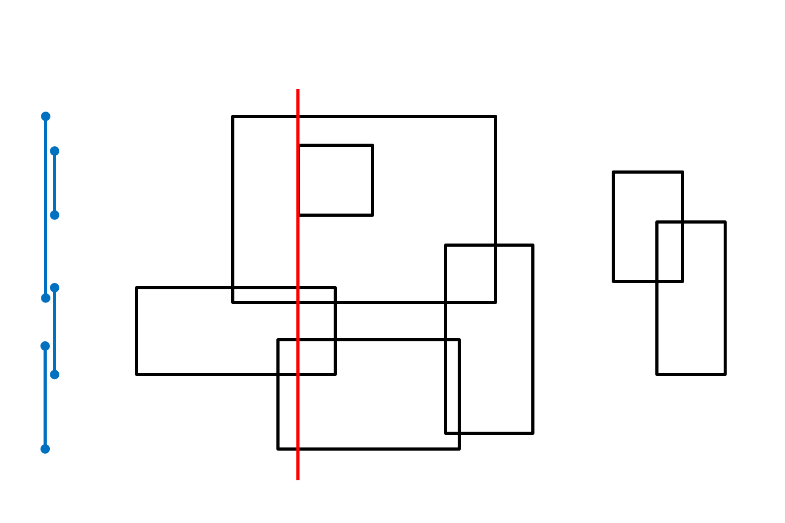
\includegraphics[scale=0.4]{images/sweep_line_8.png}
\end{center}
\end{frame}

\begin{frame}{Ejemplo visual - área de unión de rectángulos}
\begin{center}
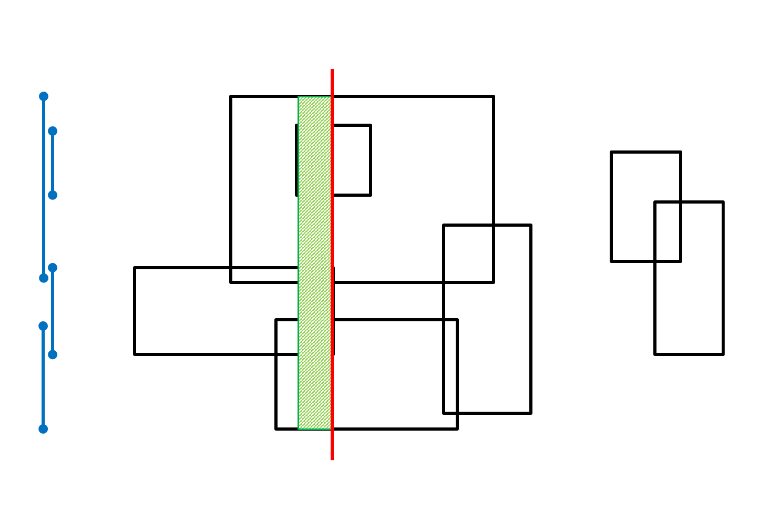
\includegraphics[scale=0.4]{images/sweep_line_9.png}
\end{center}
\end{frame}

\begin{frame}{Ejemplo visual - área de unión de rectángulos}
\begin{center}
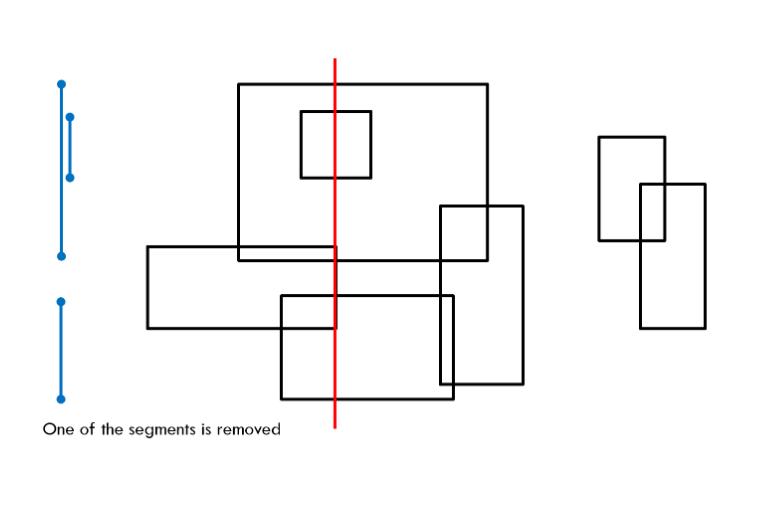
\includegraphics[scale=0.4]{images/sweep_line_10.png}
\end{center}
\end{frame}

\begin{frame}{Ejemplo visual - área de unión de rectángulos}
\begin{center}
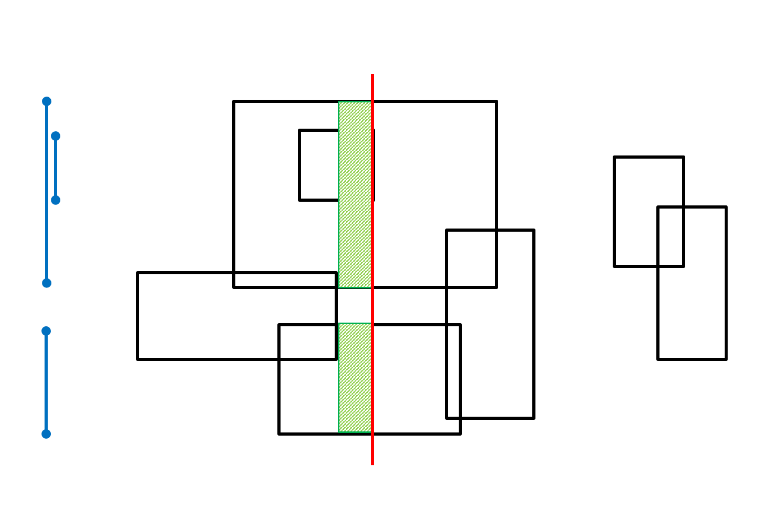
\includegraphics[scale=0.4]{images/sweep_line_11.png}
\end{center}
\end{frame}

\begin{frame}{Estructuras de datos}
La idea está clara, pero ¿qué estructura debo utilizar para poder actualizar
los segmentos rápidamente?

%%%%%%%%% TODO %%%%%%%%%

\end{frame}

\begin{frame}{Mummy Madness - WF 2011}

Nos encontramos en el desierto del Sahara, que modelamos como una grilla
formada por casillas cuadradas. Nos encontramos en el centro de una casilla
(especificada en la entrada). En cada instante nos podemos mover a cualquiera 
de las ocho casillas vecinas posibles.
\bigskip

Todo sería muy pacífico si no fuera porque varias momias se acaban de despertar:
ellas también se encuentran en los centros de algunas casillas, y en cada
paso se moverán a la casilla que más cerca esté de nosotros (en distancia euclídea).

\bigskip

¿Por cuánto tiempo podremos huir antes de que la momia nos atrape? Para este
problema, si logramos escapar del tablero de $a \times b$, estaremos salvados
para siempre.

\end{frame}

\begin{frame}{Ejemplo - Mummy Madness}

\begin{center}
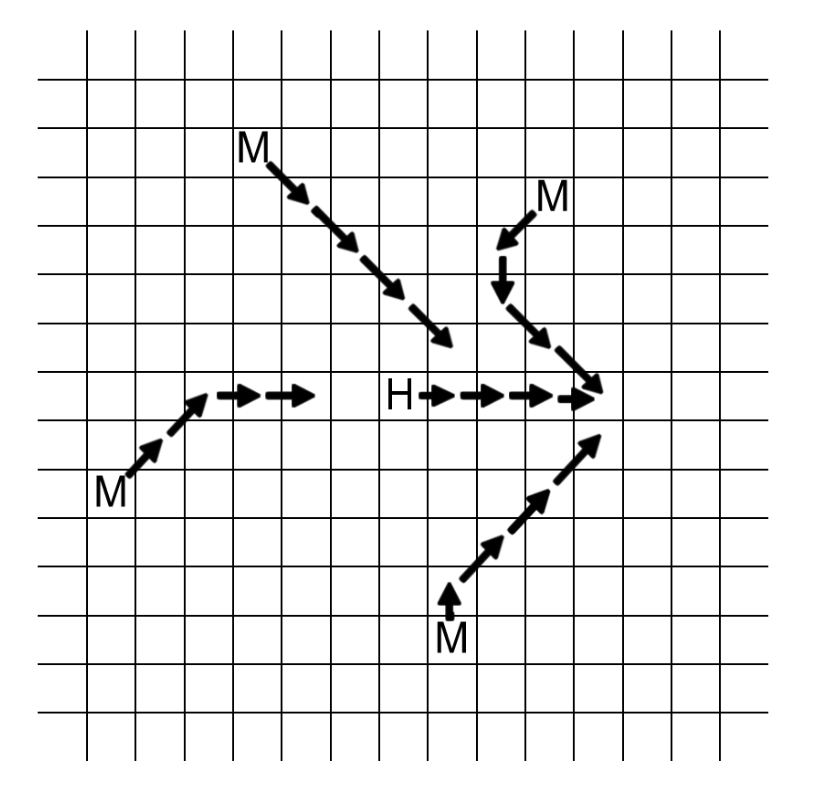
\includegraphics[scale=0.2]{images/mummy_chase.png}
\end{center}

{\footnotesize
Link al problema: \texttt{https://icpcarchive.ecs.baylor.edu/index.php?option=onlinejudge\&page=show\_problem\&problem=3137}
}
\end{frame}

\begin{frame}
Quiero ver si en tiempo $T$ existe la posibilidad de que estemos vivos o no.

\begin{block}{Observación clave}
En tiempo $T$, la persona puede encontrarse en cualquier casilla del
cuadrado de lado $2T+1$ centrado en su posición inicial. Lo mismo para
las momias (aunque está más restringido pues siguen a la persona, pero
con esto alcanza).
\end{block}

Reescribamos el problema de ver si pudimos sobrevivir hasta tiempo $T$
utilizando estos cuadrados.

\end{frame}

\begin{frame}

Lo que queremos ver es si el cuadrado formado nuestros posibles lugares
finales está cubierto completamente por la unión de los cuadrados de las 
momias. De ser así, no tenemos escapatoria. 

\bigpause

Ahora hacemos búsqueda binaria en $T$. ¿Cuál puede ser un límite superior
para la búsqueda binaria?

\end{frame}

\section{Planaridad}

\subsection{Definiciones}

\begin{frame}{Grafo planar}

\begin{block}{Definición}
    Un grafo se dice \textit{planar} si es posible dibujarlo en el plano, haciendo corresponder a cada vértice un punto, y a cada arista una curva simple continua que una los puntos correspondientes a los extremos de la arista, de manera tal que dos curvas correspondientes a aristas distintas no se intersequen más que en sus extremos.
\end{block}

\begin{block}{Definición}
    Dado un grafo planar $G$, a un dibujo de $G$ en el plano que cumple lo enunciado en la definición anterior se lo denomina un \textit{embedding}, \textit{inmersión} o simplemente \textit{dibujo} de $G$.
\end{block}

Notar que un mismo grafo planar $G$ puede tener infinitos embeddings distintos.

\end{frame}

\begin{frame}{Región}

\begin{block}{Definición}
    Dado un embedding $E$ de un grafo planar $G$, se denomina una \textit{región} de $E$ a una componente conexa del conjunto de puntos del plano que no forman parte del dibujo de $G$ en $E$.
\end{block}

Notar que al igual que muchas otras propiedades de un dibujo de un grafo planar, el conjunto de regiones depende del dibujo, y \textbf{en principio}, distintos dibujos de un mismo grafo planar podrían tener diferente cantidad de regiones.

\end{frame}

\begin{frame}{Región (cont)}

\begin{block}{Definición}
    Dada una región $f$ de un dibujo de un grafo planar $G$, se denomina el \textit{grado} de $f$ y lo notaremos $d(f)$, a la cantidad de aristas presentes en la \textit{frontera} de $f$ en el dibujo. Además, si la región $f$ toca
    a la arista de ambos lados, entonces será contada dos veces para el grado.
\end{block}

Notar que de la definición surge que cada arista ``aporta grado'' a exactamente dos regiones (o bien, a una misma región dos veces), de donde siempre se tiene $\sum_f {d(f)} = 2m$

\end{frame}

\subsection{Fórmula de Euler}

\begin{frame}{Fórmula de Euler}

La principal herramienta para trabajar con grafos planares es el siguiente resultado:

\begin{block}{Teorema}
    Si $G$ es un grafo planar conexo de $n$ vértices y $m$ aristas, y $R$ es la cantidad de regiones de \textbf{cualquier} dibujo de $G$, entonces:    
    $$R + n = m + 2 \mbox{ (fórmula de Euler)}$$
    
    En general, para un grafo planar cualquiera con $c \geq 1$ componentes conexas vale:    
    $$R + n = m + c + 1$$
\end{block}

Observar que esto es válido incluso si el grafo contiene multiejes (más de un eje entre un mismo par de nodos) y bucles (ejes de un nodo a sí mismo).

\end{frame}

\begin{frame}{Raleza de los grafos planares}

Sea $G$ un grafo simple (sin multiejes ni bucles) planar, y $g$ la longitud mínima de un ciclo simple de $g$ (si $G$ no tiene ciclos tendremos directamente $m \leq n-1$).

\begin{block}{Teorema}
    Si $G$ cumple lo anterior, entonces $m \leq \frac{(n-c-1)g}{g-2}$.
\end{block}
\begin{block}{Corolario}
    Si $G$ es grafo simple planar con $n \geq 3$, entonces $m \leq 3n - 6$.
\end{block}

Para demostrar esto, notamos que la frontera de una región debe contener un circuito, así que
$$2m = \sum_f {d(f)} \geq R g = (m-n+c+1) g \Rightarrow m \leq \frac{(n-c-1)g}{g-2}$$

\end{frame}



\begin{frame}{Ejemplos mínimos de grafos no planares}

Como consecuencia de lo anterior, notamos que:

\begin{itemize}
    \item $K_5$ no es planar: tiene $m=10$ y $n=5$, y no cumple $m \leq 3n-6$.
    \item $K_{3,3}$ no es planar: tiene $m=9$ , $n=6$ , $g=4$ y $c=1$, y no cumple $m \leq \frac{(n-c-1)g}{g-2} = \frac{(6-1-1)4}{2} = 8$.
\end{itemize}

Estos son los ejemplos no planares con menor cantidad de nodos y aristas, respectivamente.

\end{frame}

\begin{frame}{Referencias}
   \begin{itemize}
   \item \textit{Introduction to Algorithms, 2nd Edition}. MIT Press. \\ Thomas H. Cormen
   \textbf{Sección 33} (Computational Geometry)
   \item \url{https://www.topcoder.com/tc?module=Static&d1=tutorials&d2=geometry1}
   \item \url{https://www.topcoder.com/tc?module=Static&d1=tutorials&d2=geometry2}
   \item \url{https://www.topcoder.com/tc?module=Static&d1=tutorials&d2=geometry3}
   \item \url{https://www.topcoder.com/tc?module=Static&d1=tutorials&d2=lineSweep}
  \end{itemize}
  
\end{frame}

\section{Aritmética}
\begin{frame}{M\'aximo Com\'un Divisor}
\begin{block}{Definici\'on del m\'aximo com\'un divisor o $mcd$}
El m\'aximo com\'un divisor entre $a$ y $b$ o $mcd(a,b)$ ($a, b \in \mathbb{N}_0$) es el mayor n\'umero natural que los divide a ambos sin dejar resto. 
\end{block}  

Por ejemplo, $mcd(2,5) = 1$, $mcd(10,30) = 10$, $mcd(55,77) = 11$, $mcd(15,1) = 1$, $mcd(17,0) = 17$. \\
\bigskip

Notar que si $mcd(a,b) = k$ entonces $mcd(\frac{a}{k}, \frac{b}{k}) = 1$ pues quitamos todos los factores primos que eran comunes a ambos n\'umeros.

\end{frame}

\begin{frame}{Algoritmos recursivos}
	\begin{block}{Lema}
	Sea $a \leq b$ ($a, b \in \mathbb{N}_0$), entonces $mcd(a, b) = k$, $mcd(a, b-a) = k$.
	\end{block}
\bigskip

\pause
\invisible<1>{
{\small 
\textit{\textbf{Demostraci\'on:}} $mcd(a, b) = k$, luego $a = ka'$, $b = kb'$ con $mcd(a', b') = 1$. \\ \bigskip

Veamos que $mcd(a, b-a) = k$: \\
$mcd(a, b-a) = mcd(ka', kb'-ka') = mcd(ka', k(b'-a'))= k \cdot mcd(a', b'-a')$ \\ \bigskip
$\Rightarrow mcd(a, b-a) \geq k \cdot 1 = k$. Entonces seguro que $mcd(a, b-a) \geq k$, pero \textquestiondown puede suceder que $mcd(a, b-a) > k$? \\ \bigskip

Supongamos que $mcd(a, b-a) = q > k$. Entonces tenemos que:

\[ 
\left \{
  \begin{tabular}{c}
  $a \equiv 0 \pmod{q}$\\
  $b-a \equiv 0 \pmod{q}$ 
  \end{tabular}
\right.
\]
\bigskip
Luego concluimos que $a \equiv b \equiv 0 \pmod{q}$.
}
}
\end{frame}

\begin{frame}
Como $a \equiv b \equiv 0 \pmod{q}$, deducimos que $a$ y $b$ son los dos m\'ultiplos de $q$ (y recordemos que por hip\'otesis $q > k$). 
Pero luego $mcd(a,b) \geq q > k$. \\ \bigskip

\textexclamdown Absurdo pues $mcd(a,b) = k$ por hip\'otesis del ejercicio! Provino de suponer que $mcd(a, b-a) > k$. Luego, 
como $mcd(a, b-a) \leq k$ y $mcd(a, b-a) \geq k$ deducimos que $mcd(a, b-a) = k$. $\blacksquare$

\end{frame}

\begin{frame}

\begin{block}{Lema 1}
	Sea $a \leq b$ ($a, b \in \mathbb{N}_0$), entonces $mcd(a, b) = k$, $mcd(a, b-a) = k$.
\end{block}

Este lema es v\'alido como funci\'on recursiva pero puede ser mejorado. Notemos que si $b-a \geq a$, entonces al aplicar de nuevo el Lema obtendremos
$mcd(a,b-2a) = k$, y as\'i sucesivamente hasta que $b-xa < a$. Es decir que podemos mejorar el lema 1 aplic\'andolo varias veces para obtener el lema 2.\\ \bigskip

\pause
\invisible<1>{
\begin{block}{Lema 2}
{\small
	Sea $0 < a \leq b$ ($a, b \in \mathbb{N}_0$), entonces $mcd(a, b) = k$, $mcd(a, b \pmod{a}) = k$.
}
\end{block}
}
\end{frame}

\begin{frame}
\begin{block}{Lema 2}
	Sea $0 < a \leq b$ ($a, b \in \mathbb{N}_0$), entonces $mcd(a, b) = k$, $mcd(a, b \mod{a}) = k$.
\end{block}
\pause
\invisible<1>{
{\small 
\textit{\textbf{Demostraci\'on:}} \\ Como $a \leq b$, $b$ se puede escribir como $b = ra+s$ con $r, s \in \mathbb{N}_0$ y $0 \leq s < a$. \\ \bigskip
Aplicando sucesivamente el Lema 1, por inducci\'on podemos ver que $mcd(a, b-ra) = k$, pues $b - (r-1)a \geq a$ y por ende vale aplicar el lema por $r$-\'esima vez.
Ahora bien, $b-ra = s$, y $s$ es justamente el resto de $b$ m\'odulo $a$. Es decir, $s = b \mod{a}$.\\
En conclusi\'on, queda que $mcd(a,s) = k$, o en otras palabras \\ $mcd(a, b \mod{a}) = k$. $\blacksquare$
}
}
\end{frame}

\begin{frame}
Entonces ya tenemos una propiedad recursiva que nos permitir\'a hallar $mcd(a,b)$. Pero nos falta saber cu\'ando parar, es decir, los \textbf{casos base}. \\ \bigskip
\pause
\invisible<1>{
$mcd(a,0) = a$ \\
$mcd(0,a) = a$ \\ \bigskip

Notemos adem\'as que si no fueran casos base incurrir\'iamos en un error, pues $a\mod{0}$ no se puede efectuar.
}
\end{frame}

\begin{frame}[fragile]{Pseudoc\'odigo de soluci\'on recursiva}
\begin{verbatim}
function mcd (natural a, natural b) {
      if (a == 0)
           devolver b
      if (b == 0)
           devolver a
      if (a <= b)
           devolver mcd(a, b mod a)
      devolver mcd(a mod b, b)
}
\end{verbatim}
\end{frame}

\begin{frame}[fragile]{C\'odigo que tira facha}
\begin{verbatim}
int mcd (int a, int b) {
      return (a == 0) ? b : mcd(b,b\%a);
}
\end{verbatim}
\end{frame}

\begin{frame}{Demostraci\'on de complejidad}
Recordemos que en cada paso tomamos m\'odulo del n\'umero m\'as grande sobre el m\'as chico. As\'i, en cada paso obtenemos un par de n\'umeros. Como el $mcd$ es conmutativo, ponemos primero el menor n\'umero y luego el mayor. Como $a \leq b$, en dos pasos de aplicaci\'on del lema 2 se tiene que: \\ \bigskip

$mcd(a,b) = mcd(b \mod{a}, a) = mcd(a \mod{(b \mod{a})}, b \mod{a})$ \\ \bigskip

Queremos probar que el algoritmo es $O(\lg a)$, pues $a = min(a,b)$, y para ello demostraremos que cada 2 pasos del algoritmo, $a$ se reduce a la mitad.
\end{frame}

\begin{frame}{Demostraci\'on de complejidad de las implementaciones del \'item a (cont.)}
$mcd(a,b) = mcd(b \mod{a}, a) = mcd(a \mod{(b \mod{a})}, b \mod{a})$ \\ \bigskip

Queremos probar que el algoritmo es $O(\lg a)$ (pues $a = min(a,b)$) y para ello demostraremos que cada 2 pasos del algoritmo, el m\'inimo del par actual se reduce a la mitad. Si probamos eso, como cada paso es $O(1)$ y habr\'a $O(2\lg a) = O(\lg a)$ pasos, el algoritmo ser\'a $O(\lg a)$.\\ \bigskip

\end{frame}

\begin{frame}
$mcd(a,b) = mcd(b \mod{a}, a) = mcd(a \mod{(b \mod{a})}, b \mod{a})$ \\ \bigskip

\begin{enumerate}
\item Si $b \mod{a} \leq \frac{a}{2}$ entonces el m\'inimo n\'umero del par se redujo a la mitad en tan solo un paso. Como en cada paso se reduce cada n\'umero o queda igual, luego de 2 pasos el m\'inimo n\'umero del par original se habr\'a reducido a la mitad.
\item Si $b \mod{a} > \frac{a}{2}$, veamos que $a \mod{(b \mod{a})}$ ser\'a peque\~no: \\
\tabu \tabu $a = (b \mod{a})r + s$, pues $b \mod{a} < a$ (por definici\'on de m\'odulo). \\

Ahora bien, como $b \mod{a} > \frac{a}{2}$ deducimos que $r = 1$. En otras palabras, $a = (b \mod{a}) + s \Rightarrow a - (b \mod{a}) = s < a - \frac{a}{2}$, por lo que $s < \frac{a}{2}$. 
Como $s$ es por definici\'on $a \mod{(b \mod{a})}$, acabamos de ver que el menor n\'umero del par se redujo a la mitad de su valor original en dos pasos.
\end{enumerate}

\end{frame}

\end{document}
